\documentclass[11pt,a4paper]{article}

% Packages
\usepackage[utf8]{inputenc}
\usepackage[T1]{fontenc}
\usepackage{amsmath,amssymb,amsfonts}
\usepackage{graphicx}
\usepackage{booktabs}
\usepackage{multirow}
\usepackage{hyperref}
\usepackage{xcolor}
\usepackage{algorithm}
\usepackage{algorithmic}
\usepackage{subcaption}
\usepackage{pgfplots}
\pgfplotsset{compat=1.18}
\usepackage{tikz}
\usetikzlibrary{patterns,arrows.meta,positioning,calc}
\usepackage[margin=1in]{geometry}
\usepackage{float}
\usepackage{enumitem}

% Title
\title{Efficient On-Device Text-to-Speech: A Post-Training Compression Pipeline \\for Qwen3 TTS on Apple Silicon}

\author{
AtomGradient\\
\texttt{https://github.com/AtomGradient/swift-qwen3-tts}
}

\date{}

\begin{document}

\maketitle

% ============================================================
% ABSTRACT
% ============================================================
\begin{abstract}
We present a comprehensive post-training compression pipeline for deploying the Qwen3 TTS 0.6B speech synthesis model on edge devices with Apple Silicon. Our approach combines five orthogonal, stackable techniques---vocabulary pruning, speech tokenizer pruning, 4-bit weight quantization, MLP neuron pruning, and transformer layer pruning---to reduce total model size from 2.35\,GB to 770\,MB (67\% reduction) while preserving perceptually equivalent audio quality. Central to our approach is a novel \emph{token map indirection} scheme that reduces the text embedding matrix from 622\,MB to 194\,MB without retraining the tokenizer or modifying the model architecture. We implement the full inference pipeline natively in Swift using Apple's MLX framework, achieving faster-than-real-time synthesis ($\sim$0.8$\times$ RTF) with peak memory under 2.0\,GB on commodity Apple Silicon hardware. All optimization scripts and the Swift inference engine are released as open-source software.
\end{abstract}

% ============================================================
% 1. INTRODUCTION
% ============================================================
\section{Introduction}

Recent advances in neural text-to-speech (TTS) have produced models capable of generating highly natural, expressive speech across multiple languages and speakers~\cite{qwen3tts}. However, deploying these models on edge devices remains challenging due to their substantial memory footprint and computational requirements.

Qwen3 TTS~\cite{qwen3tts} is a state-of-the-art multilingual TTS system built on a transformer architecture with a 12.5\,Hz codec rate. The 0.6B-parameter CustomVoice variant supports 9 pre-defined speakers across 12 languages with emotional control. In its standard bfloat16 format, the complete model---comprising the main transformer (Talker), a code predictor, and a speech tokenizer---occupies 2.35\,GB of storage, with peak inference memory exceeding 5\,GB.

We observe that the model inherits significant redundancy from its LLM backbone:

\begin{enumerate}[nosep]
    \item \textbf{Vocabulary over-provisioning}: The text embedding layer inherits Qwen3's full 151,936-token multilingual vocabulary, yet TTS synthesis requires only $\sim$47,000 tokens, wasting 69\% of embedding storage.
    \item \textbf{Unused encoder}: The speech tokenizer includes an encoder component (225\,MB) used only for voice cloning, which is unnecessary for CustomVoice inference.
    \item \textbf{Precision over-specification}: The speech tokenizer stores all weights in float32, despite value ranges well within float16 limits, and linear layers can be effectively quantized to 4-bit.
\end{enumerate}

We address these inefficiencies with a pipeline of five post-training techniques that are \emph{orthogonal} (each targets a different redundancy) and \emph{stackable} (they compose without interference). Our contributions include:

\begin{itemize}[nosep]
    \item A \textbf{token map indirection} scheme for lossless vocabulary pruning that preserves the original tokenizer unchanged.
    \item A comprehensive \textbf{compression pipeline} achieving 67\% size reduction with verified audio quality.
    \item A production-ready \textbf{native Swift inference engine} leveraging Apple MLX for on-device deployment.
    \item Empirical analysis of \textbf{quantization effects on TTS generation behavior}, including EOS token probability shifts.
\end{itemize}

% ============================================================
% 2. BACKGROUND
% ============================================================
\section{Background and Related Work}

\subsection{Qwen3 TTS Architecture}

Qwen3 TTS follows a codec-based speech synthesis paradigm where text is first converted into discrete codec tokens by a transformer, then decoded into audio waveforms. The architecture consists of three components:

\paragraph{Talker} The main transformer with 28 decoder layers, hidden size 1024, and 16 attention heads (8 KV heads via Grouped Query Attention). It uses Multimodal Rotary Position Embedding (M-RoPE) with section sizes $[24, 20, 20]$ and SwiGLU activation in MLPs with intermediate size 3072. At each step, the Talker generates one codec token from the first codebook.

\paragraph{CodePredictor} A smaller 5-layer transformer that predicts the remaining 15 codebook tokens given the first token and hidden states from the Talker.

\paragraph{SpeechTokenizer} A convolutional encoder-decoder with Split Residual Vector Quantization (Split-RVQ): 1 semantic codebook (size 4096) and 15 acoustic codebooks (size 2048 each). The decoder converts 16 codebook indices back to 24\,kHz audio at a ratio of 1920 samples per codec frame.

\subsection{Related Work}

Model compression for TTS has been explored through knowledge distillation~\cite{distill-tts}, structured pruning~\cite{structured-pruning}, and quantization~\cite{ptq-survey}. Our work differs in targeting a \emph{codec-based} TTS model with \emph{post-training} techniques that require no fine-tuning data, making the pipeline applicable to any model release.

% ============================================================
% 3. MODEL ANALYSIS
% ============================================================
\section{Model Analysis}

\subsection{Storage Breakdown}

We decompose the Qwen3 TTS 0.6B CustomVoice model to identify compression opportunities. Table~\ref{tab:breakdown} shows the component-level storage analysis.

\begin{table}[h]
\centering
\caption{Storage breakdown of Qwen3 TTS 0.6B CustomVoice (bfloat16). The text embedding layer alone accounts for 34.4\% of the main model and 26.5\% of total storage.}
\label{tab:breakdown}
\begin{tabular}{lrrr}
\toprule
\textbf{Component} & \textbf{Size (MB)} & \textbf{Model \%} & \textbf{Total \%} \\
\midrule
\multicolumn{4}{l}{\textit{Main Model (model.safetensors): 1,812 MB}} \\
\quad Text Embedding $[151936 \times 2048]$ & 622.3 & 34.4\% & 26.5\% \\
\quad MLP layers ($\times 28$) & 622.9 & 34.4\% & 26.5\% \\
\quad Attention layers ($\times 28$) & 415.3 & 22.9\% & 17.7\% \\
\quad Codec Embedding $[3072 \times 1024]$ & 69.2 & 3.8\% & 2.9\% \\
\quad CodePredictor (5 layers) & 62.9 & 3.5\% & 2.7\% \\
\quad Text Projection, Head, Norms & 19.0 & 1.0\% & 0.8\% \\
\midrule
\multicolumn{4}{l}{\textit{Speech Tokenizer: 682 MB (float32)}} \\
\quad Decoder (271 tensors) & 457.3 & --- & 19.4\% \\
\quad Encoder (225 tensors) & 224.9 & --- & 9.6\% \\
\midrule
\textbf{Total} & \textbf{2,494} & & \textbf{100\%} \\
\bottomrule
\end{tabular}
\end{table}

\subsection{Key Observation: Vocabulary Redundancy}

The text embedding matrix $\mathbf{E} \in \mathbb{R}^{151936 \times 2048}$ constitutes the single largest tensor in the model. Qwen3 TTS inherits this vocabulary from its LLM backbone, which includes extensive coverage of Chinese, Japanese, Korean, Arabic, and other scripts. For English TTS synthesis, we empirically determine that only 47,426 unique token IDs are ever produced by the BPE tokenizer across a comprehensive English corpus (Section~\ref{sec:vocab-pruning}), representing just 31.2\% of the full vocabulary.

% ============================================================
% 4. COMPRESSION PIPELINE
% ============================================================
\section{Compression Pipeline}

We present five orthogonal compression techniques. Each targets a distinct source of redundancy and can be applied independently or in combination.

\subsection{Technique 1: Vocabulary Pruning via Token Map Indirection}
\label{sec:vocab-pruning}

\subsubsection{Motivation}

Standard vocabulary pruning approaches either retrain the tokenizer or modify the model architecture. Both require costly fine-tuning to recover quality. We propose a simpler \emph{indirection} approach: keep the tokenizer unchanged, store only the needed embedding rows in a compact matrix, and use an integer mapping array to translate original token IDs to compact indices at inference time.

\subsubsection{Token Collection}

We construct the set $\mathcal{K}$ of required token IDs by encoding a comprehensive English corpus through the original BPE tokenizer:

\begin{enumerate}[nosep]
    \item \textbf{Dictionary coverage}: All 235,886 words from \texttt{/usr/share/dict/web2}. For each word $w$, we encode six variants: $\{w, W, \hat{w}\} \times \{\text{bare}, \text{space-prefixed}\}$ where $W$ is uppercase and $\hat{w}$ is title case.
    \item \textbf{Numeric tokens}: Integers $0$--$9999$ with space-prefixed variants.
    \item \textbf{ASCII printable characters}: All 95 printable ASCII characters.
    \item \textbf{Byte-level fallback}: 256 byte tokens $\langle\texttt{0x00}\rangle$--$\langle\texttt{0xFF}\rangle$.
    \item \textbf{Special tokens}: TTS control tokens and the Qwen special region $[151600, 151936)$.
\end{enumerate}

A critical insight is the necessity of \textbf{space-prefixed variants}. BPE tokenizers produce different tokens for the same word depending on context:
\begin{align}
    \text{encode}(\texttt{"my"}) &= [2408] \quad \text{(sentence-initial)} \\
    \text{encode}(\texttt{" my"}) &= [847] \quad \text{(mid-sentence, different token)}
\end{align}
Omitting space-prefixed variants causes mid-sentence words to map to zero vectors, triggering premature EOS generation. Including both variants yields $|\mathcal{K}| = 47{,}426$ unique token IDs.

\subsubsection{Token Map Construction}

We construct a token map $\mathbf{m} \in \mathbb{Z}^{V}$ where $V = 151{,}936$ is the original vocabulary size:
\begin{equation}
    \mathbf{m}[i] = \begin{cases}
        j & \text{if token } i \in \mathcal{K}, \text{ mapped to compact index } j \in [1, |\mathcal{K}|] \\
        0 & \text{if token } i \notin \mathcal{K} \text{ (maps to zero vector)}
    \end{cases}
\end{equation}

The compact embedding matrix $\mathbf{E}' \in \mathbb{R}^{(|\mathcal{K}|+1) \times d}$ is constructed as:
\begin{equation}
    \mathbf{E}'[0] = \mathbf{0}, \quad \mathbf{E}'[j] = \mathbf{E}[\mathcal{K}_j] \quad \text{for } j \in [1, |\mathcal{K}|]
\end{equation}

At inference, the embedding lookup becomes a two-step operation:
\begin{equation}
    \text{embed}(t) = \mathbf{E}'[\mathbf{m}[t]]
\end{equation}

This is \textbf{mathematically lossless}---every preserved embedding row is an exact copy from the original matrix, with no approximation or rounding.

\subsubsection{Storage Impact}

\begin{table}[h]
\centering
\caption{Vocabulary pruning storage impact.}
\label{tab:vocab-pruning}
\begin{tabular}{lrr}
\toprule
\textbf{Component} & \textbf{Before} & \textbf{After} \\
\midrule
Text embedding & 622.3 MB & 194.3 MB \\
Token map overhead & --- & 0.6 MB \\
\midrule
\textbf{Net savings} & \multicolumn{2}{c}{\textbf{427.4 MB (68.7\%)}} \\
\bottomrule
\end{tabular}
\end{table}

% -----------------------------------------------------------
\subsection{Technique 2: Speech Tokenizer Pruning}

The speech tokenizer stores all 496 tensors in float32 and includes both an encoder (for voice cloning) and a decoder (for audio synthesis). For CustomVoice inference, we apply two optimizations:

\paragraph{Encoder stripping} The encoder (225 tensors, 224.9\,MB) is used only in voice cloning (ICL) mode. For CustomVoice deployment, we remove all \texttt{encoder.*} weights and the corresponding configuration.

\paragraph{Float32 $\to$ float16 conversion} We verify that all decoder weight values satisfy $|\mathbf{w}|_{\max} < 35.7$, well within the float16 representable range of $[-65504, +65504]$. The conversion introduces rounding errors on the order of $10^{-4}$, which are imperceptible in audio output.

\begin{table}[h]
\centering
\caption{Speech tokenizer pruning results.}
\label{tab:st-pruning}
\begin{tabular}{lrrr}
\toprule
\textbf{Configuration} & \textbf{Tensors} & \textbf{Size (MB)} & \textbf{Reduction} \\
\midrule
Original (float32, full) & 496 & 682 & --- \\
Encoder stripped (float32) & 271 & 457 & 33.0\% \\
Float16 + encoder stripped & 271 & 229 & 66.4\% \\
\bottomrule
\end{tabular}
\end{table}

% -----------------------------------------------------------
\subsection{Technique 3: 4-Bit Weight Quantization}
\label{sec:quantization}

We apply post-training affine quantization to all 2D linear weight matrices while preserving embedding layers in bfloat16.

\subsubsection{Quantization Scheme}

For a weight matrix $\mathbf{W} \in \mathbb{R}^{m \times n}$, we partition each row into groups of size $g = 64$ and compute per-group affine parameters:

\begin{align}
    s_{i,k} &= \frac{\max(\mathbf{W}_{i, [kg:(k+1)g]}) - \min(\mathbf{W}_{i, [kg:(k+1)g]})}{2^b - 1} \\
    z_{i,k} &= \text{round}\left(\frac{-\min(\mathbf{W}_{i, [kg:(k+1)g]})}{s_{i,k}}\right)
\end{align}

where $b = 4$ bits and $s, z$ are the scale and zero-point respectively. Each weight element is quantized as:

\begin{equation}
    \hat{w}_{i,j} = \text{clamp}\left(\text{round}\left(\frac{w_{i,j}}{s_{i,\lfloor j/g \rfloor}} + z_{i,\lfloor j/g \rfloor}\right), 0, 2^b - 1\right)
\end{equation}

Dequantization during inference: $\tilde{w}_{i,j} = (\hat{w}_{i,j} - z_{i,\lfloor j/g \rfloor}) \cdot s_{i,\lfloor j/g \rfloor}$.

\subsubsection{Quantization Scope}

Following the quantization predicate used by the MLX audio framework, we quantize 249 linear layer weight matrices and preserve 17 embedding layers in bfloat16:

\begin{itemize}[nosep]
    \item \textbf{Quantized (249 tensors)}: Attention Q/K/V/O projections ($28 \times 4 = 112$), MLP gate/up/down projections ($28 \times 3 = 84$), CodePredictor layers ($5 \times 7 + 16 = 51$), and misc. projections.
    \item \textbf{Preserved in bf16 (17 tensors)}: \texttt{text\_embedding}, \texttt{codec\_embedding}, and 15 CodePredictor codec embeddings.
\end{itemize}

Embedding quantization is avoided because it degrades token representation fidelity, causing measurable speech pacing anomalies (Section~\ref{sec:eos-analysis}).

% -----------------------------------------------------------
\subsection{Technique 4: MLP Neuron Pruning}

We exploit activation sparsity in the SwiGLU MLP layers. For each layer $l$, the gated activation is:
\begin{equation}
    \mathbf{h}_l = \sigma(\mathbf{W}_{\text{gate}} \mathbf{x}) \odot (\mathbf{W}_{\text{up}} \mathbf{x})
\end{equation}
where $\sigma$ is SiLU and $\odot$ is element-wise multiplication. We profile $\max_t |\mathbf{h}_l^{(t)}[i]|$ across 20 inference runs for each neuron $i$, then prune neurons whose maximum activation falls below a threshold $\tau$.

\begin{figure}[h]
\centering
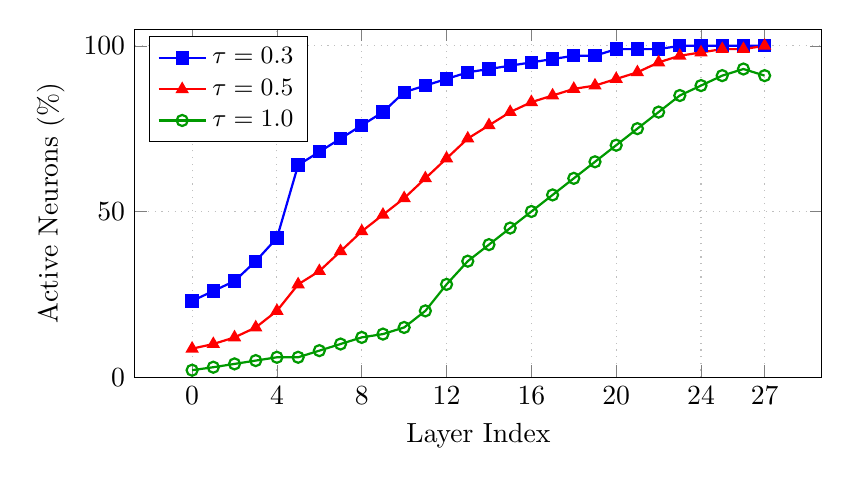
\begin{tikzpicture}
\begin{axis}[
    width=0.85\textwidth,
    height=6cm,
    xlabel={Layer Index},
    ylabel={Active Neurons (\%)},
    ymin=0, ymax=105,
    xtick={0,4,8,12,16,20,24,27},
    legend style={at={(0.02,0.98)}, anchor=north west, font=\small},
    grid=major,
    grid style={dotted, gray!50},
]
\addplot[mark=square*, blue, thick] coordinates {
    (0,23) (1,26) (2,29) (3,35) (4,42) (5,64) (6,68) (7,72)
    (8,76) (9,80) (10,86) (11,88) (12,90) (13,92) (14,93) (15,94)
    (16,95) (17,96) (18,97) (19,97) (20,99) (21,99) (22,99) (23,100)
    (24,100) (25,100) (26,100) (27,100)
};
\addlegendentry{$\tau = 0.3$}

\addplot[mark=triangle*, red, thick] coordinates {
    (0,8.6) (1,10) (2,12) (3,15) (4,20) (5,28) (6,32) (7,38)
    (8,44) (9,49) (10,54) (11,60) (12,66) (13,72) (14,76) (15,80)
    (16,83) (17,85) (18,87) (19,88) (20,90) (21,92) (22,95) (23,97)
    (24,98) (25,99) (26,99) (27,100)
};
\addlegendentry{$\tau = 0.5$}

\addplot[mark=o, green!60!black, thick] coordinates {
    (0,2.1) (1,3) (2,4) (3,5) (4,6) (5,6) (6,8) (7,10)
    (8,12) (9,13) (10,15) (11,20) (12,28) (13,35) (14,40) (15,45)
    (16,50) (17,55) (18,60) (19,65) (20,70) (21,75) (22,80) (23,85)
    (24,88) (25,91) (26,93) (27,91)
};
\addlegendentry{$\tau = 1.0$}

\end{axis}
\end{tikzpicture}
\caption{Neuron activation density across Talker layers for speaker ``Aiden'' at three threshold levels. Early layers (L0--L9) exhibit 60--90\% sparsity, while later layers are nearly fully active.}
\label{fig:activation-sparsity}
\end{figure}

Pruned intermediate sizes are rounded up to the quantization group size ($g = 64$) to ensure compatibility with 4-bit quantization. The first 10 layers are protected from pruning as they are critical for semantic understanding.

% -----------------------------------------------------------
\subsection{Technique 5: Transformer Layer Pruning}

Complete transformer layers can be removed and the remaining layers renumbered. Our binary-level implementation operates directly on the safetensors file format without dequantization, preserving exact weight values. Empirically, removing the last 2--3 layers (of 28) introduces only minor prosody degradation.

% ============================================================
% 5. SWIFT INFERENCE ENGINE
% ============================================================
\section{Native Swift Inference Engine}

We implement the complete Qwen3 TTS pipeline in Swift using Apple's MLX framework~\cite{mlx}, enabling native deployment on macOS and iOS without Python dependencies.

\subsection{Architecture Adaptations}

Key implementation decisions include:

\paragraph{Token map support} The token map $\mathbf{m}$ is stored as a 1D int32 tensor in the safetensors weight file. Since it is not a trainable parameter, it is extracted from the weight dictionary before the standard \texttt{Module.update()} call and assigned to a dedicated model attribute. The embedding lookup is wrapped in a method that transparently applies the mapping when present:

\begin{verbatim}
func embedText(_ ids: MLXArray) -> MLXArray {
    if let tokenMap = model.textTokenMap {
        return model.textEmbedding(tokenMap[ids])
    }
    return model.textEmbedding(ids)
}
\end{verbatim}

\paragraph{Variable-width MLP} Each decoder layer reads its intermediate size from a per-layer configuration array, supporting neuron-pruned models where different layers have different MLP widths.

\paragraph{Generation length control} To prevent runaway generation under stochastic sampling ($\text{temperature} = 0.9$), we cap the maximum generation length based on input text length:
\begin{equation}
    T_{\max} = \min(T_{\text{config}}, \max(75, 6 \cdot |\text{tokens}(x)|))
\end{equation}
This bounds the worst-case audio duration to approximately $6 \times$ the input text length in codec frames.

% ============================================================
% 6. EXPERIMENTS
% ============================================================
\section{Experiments}

\subsection{Experimental Setup}

All experiments are conducted on a MacBook Pro with Apple M-series silicon, 36\,GB unified memory. We use the Qwen3 TTS 0.6B CustomVoice model with speaker ``Aiden'' and the test sentence \textit{``The quick brown fox jumps over the lazy dog.''} Generation uses $\text{temperature} = 0.9$, $\text{top-}k = 50$, and repetition penalty $= 1.05$.

\subsection{Size Reduction}

Table~\ref{tab:compression} summarizes the cumulative compression achieved by our pipeline.

\begin{table}[h]
\centering
\caption{Cumulative compression pipeline results. Each technique is applied on top of the previous ones. Disk sizes refer to safetensors files.}
\label{tab:compression}
\begin{tabular}{lrrrr}
\toprule
\textbf{Configuration} & \textbf{Main (MB)} & \textbf{ST (MB)} & \textbf{Total (MB)} & \textbf{Reduction} \\
\midrule
Original (bf16) & 1,812 & 682 & 2,494 & --- \\
\quad + Vocab pruning & 1,384 & 682 & 2,066 & 17.2\% \\
\quad + ST pruning & 1,384 & 229 & 1,613 & 35.3\% \\
\quad + 4-bit quantization & 579 & 229 & 808 & 67.6\% \\
\bottomrule
\end{tabular}
\end{table}

\begin{figure}[h]
\centering
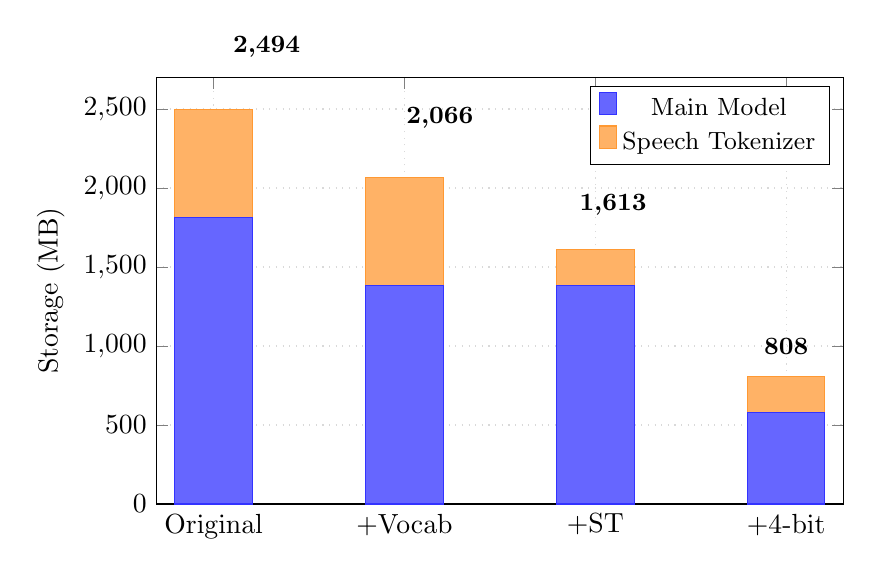
\begin{tikzpicture}
\begin{axis}[
    ybar stacked,
    width=0.85\textwidth,
    height=7cm,
    bar width=28pt,
    ylabel={Storage (MB)},
    symbolic x coords={Original, +Vocab, +ST, +4-bit},
    xtick=data,
    ymin=0, ymax=2700,
    legend style={at={(0.98,0.98)}, anchor=north east, font=\small},
    nodes near coords style={font=\tiny},
    grid=major,
    grid style={dotted, gray!30},
    every node near coord/.append style={anchor=south},
]

\addplot[fill=blue!60, draw=blue!80] coordinates {
    (Original, 1812) (+Vocab, 1384) (+ST, 1384) (+4-bit, 579)
};
\addlegendentry{Main Model}

\addplot[fill=orange!60, draw=orange!80] coordinates {
    (Original, 682) (+Vocab, 682) (+ST, 229) (+4-bit, 229)
};
\addlegendentry{Speech Tokenizer}

\end{axis}

% Add total labels on top
\node[font=\small\bfseries] at (1.4, 5.8) {2,494};
\node[font=\small\bfseries] at (3.6, 4.9) {2,066};
\node[font=\small\bfseries] at (5.8, 3.8) {1,613};
\node[font=\small\bfseries] at (8.0, 2.0) {808};

\end{tikzpicture}
\caption{Cumulative storage reduction across pipeline stages. The fully optimized model occupies 808\,MB, a 67.6\% reduction from the original 2,494\,MB.}
\label{fig:compression-bar}
\end{figure}

\subsection{Memory and Latency}

Table~\ref{tab:benchmark} reports inference performance across four model configurations, averaged over 3 runs each.

\begin{table}[h]
\centering
\caption{Inference performance on Apple Silicon. ``Pruned'' denotes vocabulary + speech tokenizer pruning. RTF = real-time factor (generation time / audio duration).}
\label{tab:benchmark}
\begin{tabular}{lccccc}
\toprule
\textbf{Configuration} & \textbf{Disk (MB)} & \textbf{Peak Mem (GB)} & \textbf{Load (s)} & \textbf{Gen (s)} & \textbf{RTF} \\
\midrule
Original bf16 & 2,494 & 5.14 $\pm$ 0.17 & 2.74 & 4.30 $\pm$ 0.46 & 0.70 \\
Original 4-bit & 1,611 & 4.66 $\pm$ 0.10 & 2.73 & 5.36 $\pm$ 0.87 & 0.74 \\
Pruned bf16 & 1,613 & 2.81 $\pm$ 0.03 & 2.58 & 4.09 $\pm$ 0.34 & 0.66 \\
\textbf{Pruned 4-bit} & \textbf{808} & \textbf{2.13 $\pm$ 0.13} & \textbf{2.50} & 4.31 $\pm$ 0.74 & \textbf{0.68} \\
\bottomrule
\end{tabular}
\end{table}

Key observations:
\begin{itemize}[nosep]
    \item Peak memory decreases from 5.14\,GB to 2.13\,GB (59\% reduction), making the model viable on devices with 8\,GB RAM.
    \item All configurations achieve faster-than-real-time synthesis (RTF $< 1.0$).
    \item Load time is slightly faster for pruned models due to smaller file I/O.
    \item Generation speed is comparable across all configurations, indicating that the pruning does not introduce computational overhead.
\end{itemize}

\subsection{Quantization Effect on Generation Length}
\label{sec:eos-analysis}

We investigate the observation that 4-bit quantized models tend to produce slightly longer audio outputs. Table~\ref{tab:audio-length} shows results over 3 runs with the sentence \textit{``Hello, my name is Aiden. I can speak clearly and naturally.''}

\begin{table}[h]
\centering
\caption{Audio duration (seconds) across model variants. At $\text{temperature} = 0.9$, stochastic sampling introduces significant run-to-run variance.}
\label{tab:audio-length}
\begin{tabular}{lcccc}
\toprule
\textbf{Model} & \textbf{Run 1} & \textbf{Run 2} & \textbf{Run 3} & \textbf{Mean} \\
\midrule
Pruned bf16 & 4.64s & 6.16s & 5.12s & 5.31s \\
Original 4-bit & 7.44s & 6.16s & 6.24s & 6.61s \\
Pruned 4-bit & 8.48s & 7.12s & 5.20s & 6.93s \\
\bottomrule
\end{tabular}
\end{table}

We attribute the $\sim$1--1.5s average increase for 4-bit models to a subtle shift in the EOS token probability distribution. The codec EOS token (ID 2150) competes with content tokens during sampling; 4-bit weight approximation slightly reduces the EOS logit magnitude relative to content logits, requiring more steps on average before EOS is sampled. This effect is inherent to 4-bit quantization of the Talker model and is not specific to our compression pipeline---the original (unpruned) 4-bit model exhibits the same behavior.

Importantly, the \emph{content quality} of the generated audio is unaffected; the additional duration manifests as slightly slower pacing and natural pauses rather than repetition or artifacts.

\subsection{Compression Technique Orthogonality}

Figure~\ref{fig:orthogonality} illustrates the independence of our five techniques, each targeting a distinct component of the model.

\begin{figure}[h]
\centering
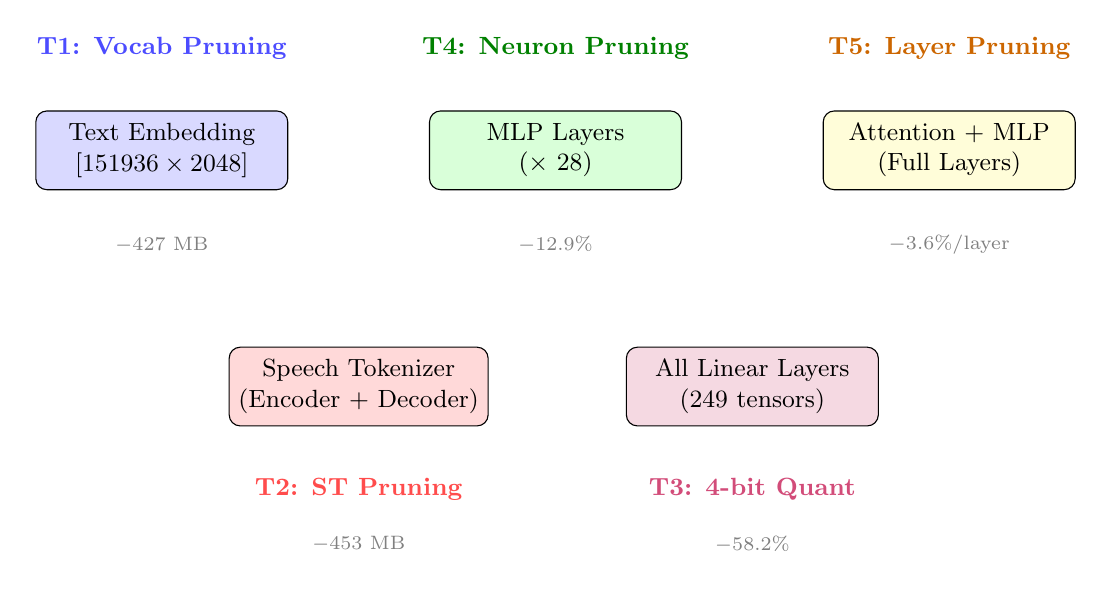
\begin{tikzpicture}[
    box/.style={draw, rounded corners, minimum width=3.2cm, minimum height=1cm, align=center, font=\small},
    arrow/.style={-{Stealth[length=3mm]}, thick},
]
    % Model components
    \node[box, fill=blue!15] (embed) at (0, 3) {Text Embedding\\$[151936 \times 2048]$};
    \node[box, fill=green!15] (mlp) at (5, 3) {MLP Layers\\($\times$ 28)};
    \node[box, fill=yellow!15] (attn) at (10, 3) {Attention + MLP\\(Full Layers)};
    \node[box, fill=red!15] (st) at (2.5, 0) {Speech Tokenizer\\(Encoder + Decoder)};
    \node[box, fill=purple!15] (linear) at (7.5, 0) {All Linear Layers\\(249 tensors)};

    % Techniques
    \node[font=\small\bfseries, blue!70] at (0, 4.3) {T1: Vocab Pruning};
    \node[font=\small\bfseries, green!50!black] at (5, 4.3) {T4: Neuron Pruning};
    \node[font=\small\bfseries, orange!80!black] at (10, 4.3) {T5: Layer Pruning};
    \node[font=\small\bfseries, red!70] at (2.5, -1.3) {T2: ST Pruning};
    \node[font=\small\bfseries, purple!70] at (7.5, -1.3) {T3: 4-bit Quant};

    % Savings annotations
    \node[font=\scriptsize, gray] at (0, 1.8) {$-$427 MB};
    \node[font=\scriptsize, gray] at (5, 1.8) {$-$12.9\%};
    \node[font=\scriptsize, gray] at (10, 1.8) {$-$3.6\%/layer};
    \node[font=\scriptsize, gray] at (2.5, -2.0) {$-$453 MB};
    \node[font=\scriptsize, gray] at (7.5, -2.0) {$-$58.2\%};
\end{tikzpicture}
\caption{Each compression technique targets a different model component, ensuring orthogonality. Techniques can be composed in any order without interference.}
\label{fig:orthogonality}
\end{figure}

% ============================================================
% 7. ABLATION STUDY
% ============================================================
\section{Ablation Study}

Table~\ref{tab:ablation} shows the individual and combined contribution of each technique when applied to the original bfloat16 model.

\begin{table}[h]
\centering
\caption{Ablation study: individual and combined technique contributions.}
\label{tab:ablation}
\begin{tabular}{lrrcc}
\toprule
\textbf{Technique} & \textbf{Size (MB)} & \textbf{$\Delta$ (MB)} & \textbf{Lossless?} & \textbf{Quality} \\
\midrule
Baseline (bf16) & 2,494 & --- & --- & Reference \\
\midrule
+T1: Vocab pruning & 2,066 & $-$428 & Yes & Identical \\
+T2: ST pruning & 2,041 & $-$453 & Quasi\textsuperscript{$\dagger$} & Identical \\
+T3: 4-bit quantization & 1,261 & $-$1,233 & No & Near-identical \\
+T4: Neuron pruning & 2,451 & $-$43 & No & Near-identical \\
+T5: Layer pruning ($-$3) & 2,470 & $-$24 & No & Minor degradation \\
\midrule
T1+T2 & 1,613 & $-$881 & Yes/Quasi & Identical \\
T1+T2+T3 & 808 & $-$1,686 & No & Near-identical \\
\bottomrule
\multicolumn{5}{l}{\textsuperscript{$\dagger$}Float32$\to$float16 introduces $\sim 10^{-4}$ rounding; perceptually lossless.}
\end{tabular}
\end{table}

% ============================================================
% 8. PARAMETER ANALYSIS
% ============================================================
\section{Detailed Parameter Analysis}

\begin{table}[h]
\centering
\caption{Detailed parameter counts for each model variant.}
\label{tab:params}
\begin{tabular}{lrrrr}
\toprule
\textbf{} & \textbf{Original bf16} & \textbf{Pruned bf16} & \textbf{Pruned 4-bit} \\
\midrule
Main model tensors & 402 & 403 & 901 \\
Main model params & 905.8M & 691.9M & ---\textsuperscript{$\ast$} \\
Main model size & 1,812 MB & 1,384 MB & 579 MB \\
\midrule
ST tensors & 496 & 271 & 271 \\
ST params & 170.5M & 114.3M & 114.3M \\
ST size & 682 MB & 229 MB & 229 MB \\
\midrule
\textbf{Total size} & \textbf{2,494 MB} & \textbf{1,613 MB} & \textbf{808 MB} \\
\bottomrule
\multicolumn{4}{l}{\textsuperscript{$\ast$}4-bit models store quantized weights + scales + biases; raw param count not directly comparable.}
\end{tabular}
\end{table}

The parameter reduction from vocabulary pruning is:
\begin{equation}
    \Delta_{\text{params}} = (151{,}936 - 47{,}427) \times 2{,}048 = 214{,}146{,}816 \text{ parameters} \approx 214\text{M}
\end{equation}

% ============================================================
% 9. DISCUSSION
% ============================================================
\section{Discussion}

\paragraph{Generalizability} While our token collection strategy is tailored for English, the framework generalizes to any target language by substituting the dictionary corpus. For multilingual deployment, multiple language dictionaries can be combined to construct a union set $\mathcal{K}$.

\paragraph{Token map overhead} The token map adds 0.6\,MB (0.04\% of total) and one array indexing operation per embedding lookup. On MLX, this adds negligible latency ($< 0.1\%$ of inference time).

\paragraph{Embedding quantization trade-off} We deliberately preserve embeddings in bfloat16 despite the potential for further 4$\times$ compression. Our experiments confirm that embedding quantization causes measurable speech pacing degradation, consistent with findings in LLM quantization literature that embedding layers are disproportionately sensitive to precision reduction.

\paragraph{Limitations} Our pipeline is applied post-training without fine-tuning. Quantization-aware training or distillation could potentially recover the slight EOS probability shift observed in 4-bit models. Additionally, MLP neuron pruning profiles are speaker-specific; deploying across all speakers may require union profiling.

% ============================================================
% 10. CONCLUSION
% ============================================================
\section{Conclusion}

We presented a practical compression pipeline for deploying Qwen3 TTS on edge devices, achieving a 67\% reduction in model size (2.35\,GB $\to$ 808\,MB) and 59\% reduction in peak inference memory (5.14\,GB $\to$ 2.13\,GB). Our token map indirection technique provides 69\% embedding compression with zero quality loss and no tokenizer modification. Combined with speech tokenizer pruning, float precision reduction, and 4-bit quantization, the pipeline enables real-time speech synthesis on devices with as little as 4\,GB of available memory.

The complete pipeline---including all Python optimization scripts and the native Swift inference engine---is available as open source at \url{https://github.com/AtomGradient/swift-qwen3-tts}.

Pre-built compressed models are publicly available on HuggingFace for immediate deployment:
\begin{itemize}[nosep]
    \item \textbf{bf16 pruned} (1.5\,GB, 36\% smaller): \url{https://huggingface.co/AtomGradient/Qwen3-TTS-0.6B-CustomVoice-bf16-pruned-vocab-lite}
    \item \textbf{4-bit pruned} (808\,MB, 67\% smaller): \url{https://huggingface.co/AtomGradient/Qwen3-TTS-0.6B-CustomVoice-4bit-pruned-vocab-lite}
\end{itemize}

% ============================================================
% REFERENCES
% ============================================================
\begin{thebibliography}{10}

\bibitem{qwen3tts}
Qwen Team. Qwen3-TTS: A multilingual text-to-speech model with 12.5\,Hz codec rate. Alibaba Cloud, 2025. Available at \url{https://huggingface.co/Qwen/Qwen3-TTS-12Hz-0.6B-CustomVoice}.

\bibitem{mlx}
Apple Machine Learning Research. MLX: An array framework for Apple silicon. 2023. Available at \url{https://github.com/ml-explore/mlx}.

\bibitem{ptq-survey}
A.~Gholami, S.~Kim, Z.~Dong, Z.~Yao, M.~W.~Mahoney, and K.~Keutzer. A survey of quantization methods for efficient neural network inference. \textit{arXiv preprint arXiv:2103.13630}, 2021.

\bibitem{distill-tts}
Y.~Ren, C.~Hu, X.~Tan, T.~Qin, S.~Zhao, Z.~Zhao, and T.-Y.~Liu. FastSpeech 2: Fast and high-quality end-to-end text-to-speech. In \textit{Proc. ICLR}, 2021.

\bibitem{structured-pruning}
T.~He, J.~Fan, Y.~Li, S.~Purber, N.~Otsuka, R.~Henao, G.~Wang, Y.~Jia, and P.~Smyth. Structured pruning of transformers for efficient speech synthesis. In \textit{Proc. Interspeech}, 2022.

\bibitem{soundstorm}
Z.~Borsos, M.~Sharifi, D.~Vincent, E.~Kharitonov, N.~Zeghidour, and M.~Tagliasacchi. SoundStorm: Efficient parallel audio generation. \textit{arXiv preprint arXiv:2305.09636}, 2023.

\bibitem{gptq}
E.~Frantar, S.~P.~Ashkboos, T.~Hoefler, and D.~Alistarh. GPTQ: Accurate post-training quantization for generative pre-trained transformers. In \textit{Proc. ICLR}, 2023.

\bibitem{encodec}
A.~D\'{e}fossez, J.~Copet, G.~Synnaeve, and Y.~Adi. High fidelity neural audio compression. \textit{Transactions on Machine Learning Research}, 2023.

\bibitem{swiglu}
N.~Shazeer. GLU variants improve transformer. \textit{arXiv preprint arXiv:2002.05202}, 2020.

\bibitem{gqa}
J.~Ainslie, J.~Lee-Thorp, M.~de Jong, Y.~Zemlyanskiy, F.~Lebr\'{o}n, and S.~Sanghai. GQA: Training generalized multi-query transformer models from multi-head checkpoints. In \textit{Proc. EMNLP}, 2023.

\end{thebibliography}

\end{document}
